% Synthetic preview only. Replace mock_results.json with measured results.
\begin{figure*}[t]
  \centering
  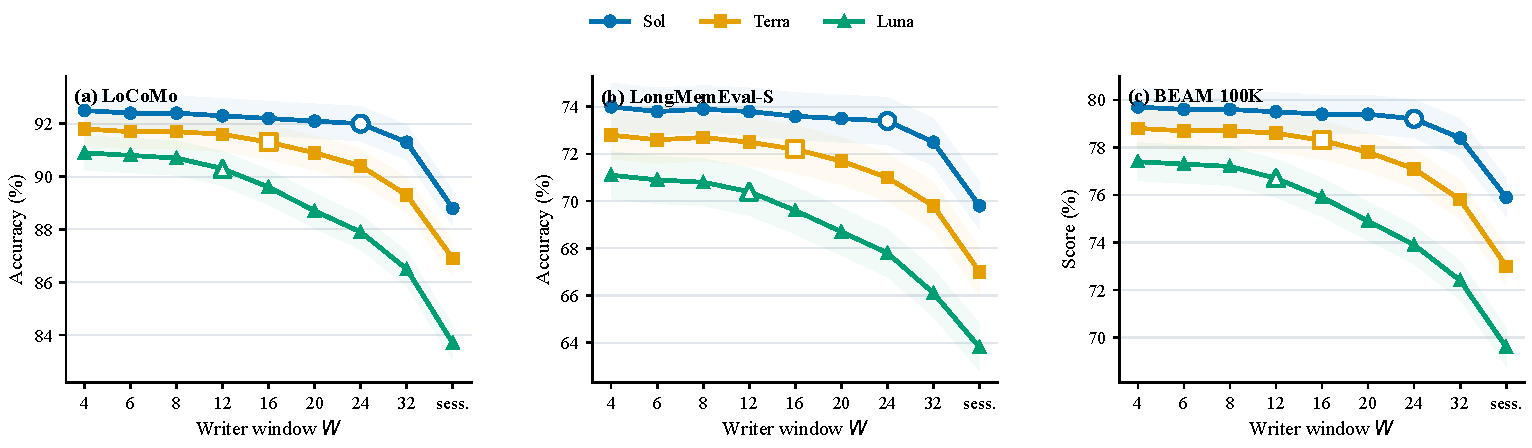
\includegraphics[width=\textwidth]{figures/mock_gpt56_chunk_curve/fig1_quality_curves.pdf}
  \caption{Hypothetical effect of Writer input granularity on downstream memory quality. Open markers identify the selected model-specific window. Shaded regions denote illustrative 95\% confidence intervals.}
  \label{fig:mock_quality_curves}
\end{figure*}

\begin{figure*}[t]
  \centering
  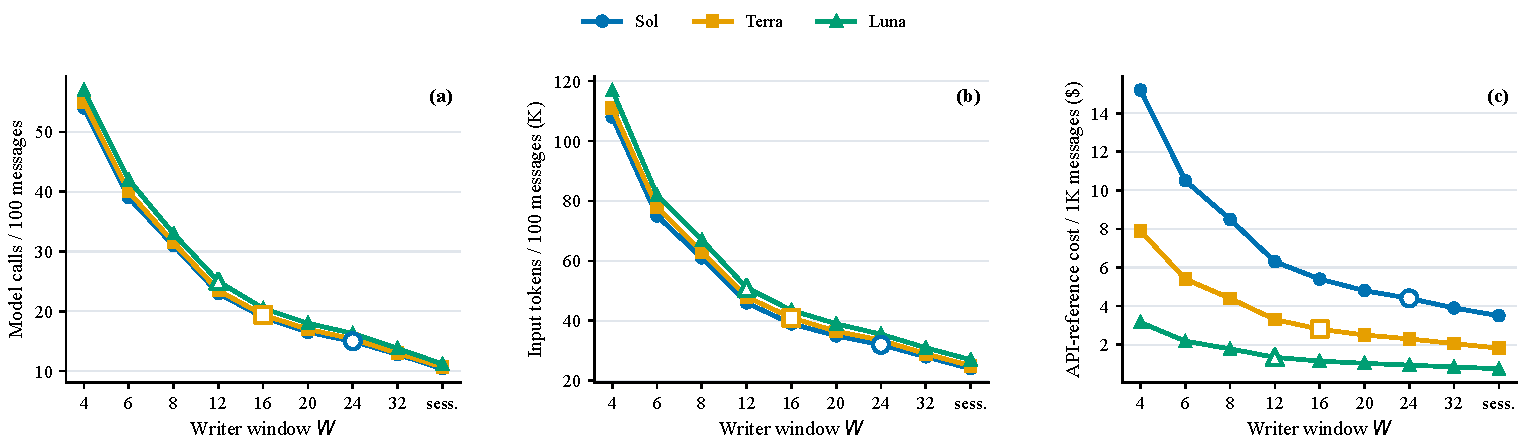
\includegraphics[width=\textwidth]{figures/mock_gpt56_chunk_curve/fig2_cost_curves.pdf}
  \caption{Hypothetical memory-construction cost as the Writer window increases. Costs include Writer, Verify, and Tidy calls. Dollar values use API-reference pricing and are not subscription charges.}
  \label{fig:mock_cost_curves}
\end{figure*}

\begin{figure}[t]
  \centering
  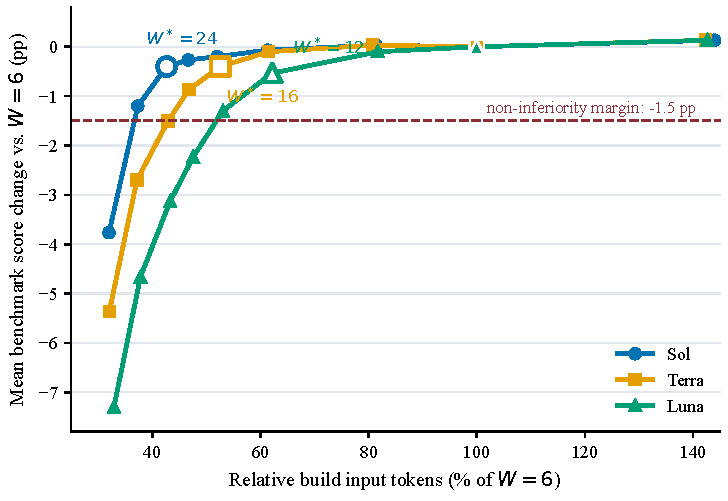
\includegraphics[width=0.49\textwidth]{figures/mock_gpt56_chunk_curve/fig3_quality_cost_pareto.pdf}
  \caption{Hypothetical quality--cost trade-off. Each open marker is the largest model-specific window satisfying the pre-registered non-inferiority criterion.}
  \label{fig:mock_quality_cost}
\end{figure}

\begin{table*}[t]
\centering
\caption{Hypothetical full-benchmark results after selecting the Writer window on a disjoint development subset. All values are synthetic placeholders. Calls, tokens, cost, and latency cover memory construction only.}
\label{tab:mock_chunk_main}
\small
\begin{tabular}{llrrrrrrr}
\toprule
Writer & $W$ & LoCoMo & LongMemEval-S & BEAM & Calls/100 & Tokens/100 (K) & \$/1K & Min/1K \\
\midrule
Sol & 6 & 92.4 & 73.8 & 79.6 & 39.0 & 75.0 & 10.50 & 84.0 \\
\textbf{Sol} & \textbf{24} & \textbf{92.0} & \textbf{73.4} & \textbf{79.2} & \textbf{15.0} & \textbf{32.0} & \textbf{4.40} & \textbf{36.8} \\
Sol & session & 88.8 & 69.8 & 75.9 & 10.4 & 24.0 & 3.50 & 28.9 \\
\midrule
Terra & 6 & 91.7 & 72.6 & 78.7 & 40.0 & 78.0 & 5.40 & 79.2 \\
\textbf{Terra} & \textbf{16} & \textbf{91.3} & \textbf{72.2} & \textbf{78.3} & \textbf{19.4} & \textbf{41.0} & \textbf{2.80} & \textbf{41.5} \\
Terra & session & 86.9 & 67.0 & 73.0 & 10.7 & 25.0 & 1.82 & 27.5 \\
\midrule
Luna & 6 & 90.8 & 70.9 & 77.3 & 42.0 & 82.0 & 2.18 & 74.5 \\
\textbf{Luna} & \textbf{12} & \textbf{90.3} & \textbf{70.4} & \textbf{76.7} & \textbf{25.0} & \textbf{51.0} & \textbf{1.34} & \textbf{47.0} \\
Luna & session & 83.7 & 63.8 & 69.6 & 11.2 & 27.0 & 0.75 & 25.8 \\
\bottomrule
\end{tabular}
\end{table*}

\begin{table}[t]
\centering
\caption{Hypothetical model-specific window selection. A configuration passes when the lower 95\% confidence bound exceeds $-1.5$ points and construction cost falls by at least 20\%.}
\label{tab:mock_chunk_selection}
\small
\begin{tabular}{lrrrrrr}
\toprule
Writer & $W^*$ & $\Delta$Score & CI lower & Calls $\downarrow$ & Tokens $\downarrow$ & Cost $\downarrow$ \\
\midrule
Sol & 24 & -0.4 & -1.0 & 61.5\% & 57.3\% & 58.1\% \\
Terra & 16 & -0.4 & -1.2 & 51.5\% & 47.4\% & 48.1\% \\
Luna & 12 & -0.5 & -1.4 & 40.5\% & 37.8\% & 38.5\% \\
\bottomrule
\end{tabular}
\end{table}

